% The preamble
\documentclass{article}
\pagestyle{plain} %includes page numbers

\usepackage[margin=1in]{geometry} %included to change page margins
\usepackage{graphicx} %included to insert a graph
\usepackage{caption} %included to include a caption over the graph
\usepackage{booktabs} %needed for the table's toprule midrule and bottomrule sequences
\usepackage[section]{placeins} %to keep graphs and tables in the very section to which they belong 
\usepackage{pdflscape} %to include the landscape environment 

\title{My third document}
\author{Jane Doe}
\date{31 September 2016}

% The body
\begin{document}
\maketitle
\tableofcontents{}
\listoffigures{}
\listoftables{}

\section{Lists}
\subsection{Numbering}
\begin{enumerate}
	\item The first point
	\item The second point
	\item The third point
\end{enumerate}

\subsection{Bullet Points}
\begin{itemize}
	\item The first point
	\item The second point
	\item The third point
\end{itemize}

\subsection{Nesting}
{\textbf{
	\begin{enumerate}
		\item Note that you can include as many environments within environments...
		\item and lists within lists.
		\begin{enumerate}
			\item Level 2 item 
			\begin{itemize}
				\item Level 3 item
			\end{itemize} 
		\end{enumerate}
	\end{enumerate}
}}

\section{Graphs}

\begin{center}
	\begin{figure}[h]
		\caption{A Lion}
		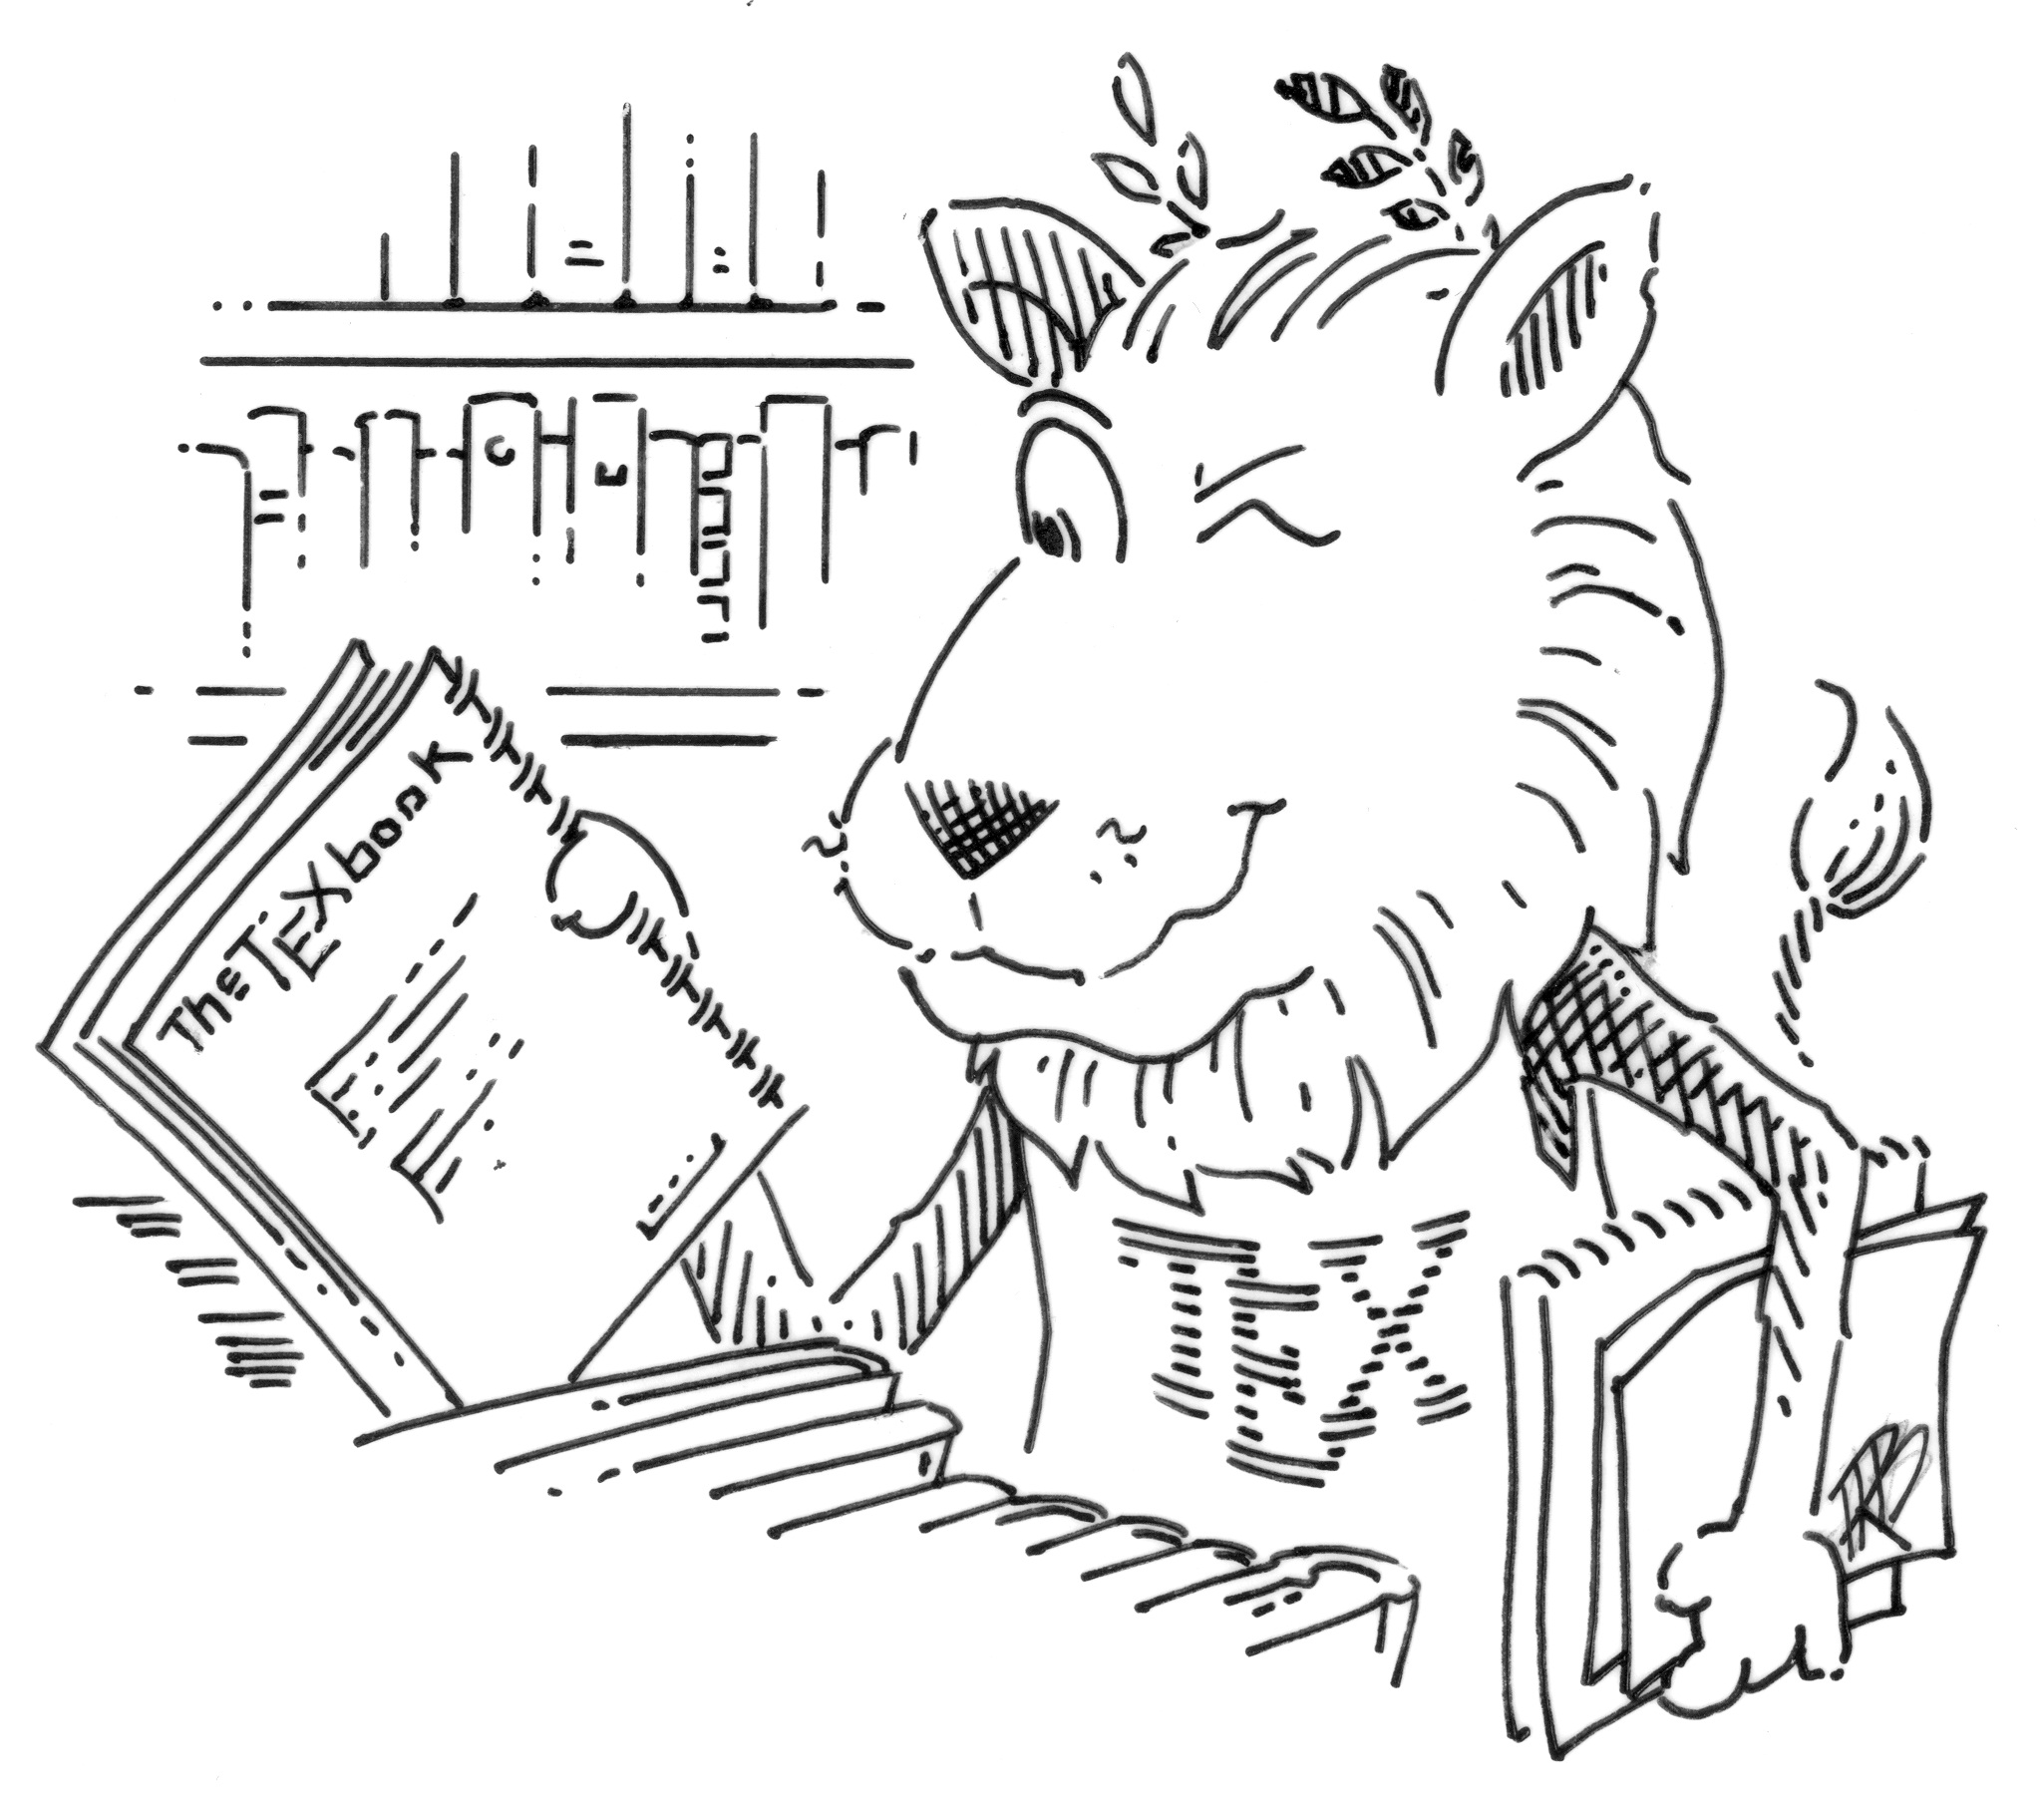
\includegraphics[scale=0.07]{ctan_lion_600.jpg}
	\end{figure}
\end{center}

\begin{landscape}
\section{Tables}

{\small{
% Table generated by Excel2LaTeX '
\begin{table}[]
  \centering
  \caption{Explaining low take-up}
    \begin{tabular}{rrrrr}
    \toprule
    \textbf{Summary statistics regarding hypothesis 2} &       &       &       &  \\
    \midrule
          &       & \multicolumn{1}{c}{(1)} & \multicolumn{1}{c}{(2)} & \multicolumn{1}{c}{(3)} \\
          &       & Take-up &       & \multicolumn{1}{c}{\textit{p-val}} \\
          & \multicolumn{1}{c}{All} & \multicolumn{1}{c}{No} & \multicolumn{1}{c}{Yes} & \multicolumn{1}{c}{No = Yes} \\
    \textbf{Government transfers} &       &       &       &  \\
    Has a Ficha de Protecci\'{o}n Social & 90.41\% & 89.97\% & 97.30\% & 0.142 \\
          &       &       &       &  \\
    Beneficiary of Programa Puente / Chile Solidario & 14.94\% & 14.34\% & 24.32\% & 0.098 \\
          &       &       &       &  \\
    Household receives government assistance & 73.20\% & 73.57\% & 67.57\% & 0.425 \\
          &       &       &       &  \\
    Household receives some type of pension & 31.60\% & 32.06\% & 24.32\% & 0.326 \\
          &       &       &       &  \\
    Household receives any sort of (non-)monetary government assistance** & 65.81\% & 66.04\% & 62.16\% & 0.630 \\
          &       &       &       &  \\
    Active beneficiary of the government's PUENTE program** & 14.35\% & 14.21\% & 16.67\% & 0.684 \\
    \bottomrule
    \end{tabular}%
  \label{tab:addlabel}%
\end{table}%
}} % Ending the small text font
\end{landscape}%

\end{document}
